\subsection{AGC Block Diagrams}
The AGC process is shown in Figures \ref{fig: agc block diagram 1}, \ref{fig: agc block diagram 2}, and \ref{fig: agc block diagram 3}.
$RACE$ (reporting ACE) and SACE (smoothed ACE) are calculated using PU values assuming $B$ is a positive non-PU value with units of $MW/0.1Hz$.
If $K_{bv}$ is not zero, the resulting $RACE$ is not the industry standard (WECC defined) $RACE$ value.
The scheduled interchange may be altered by the user via a \verb|mAGC_sig| file that controls the behavior of the $IC_{adj}$ input.

% NOTE: say something about an example?

\begin{figure}[!h]
	\centering
	\footnotesize
	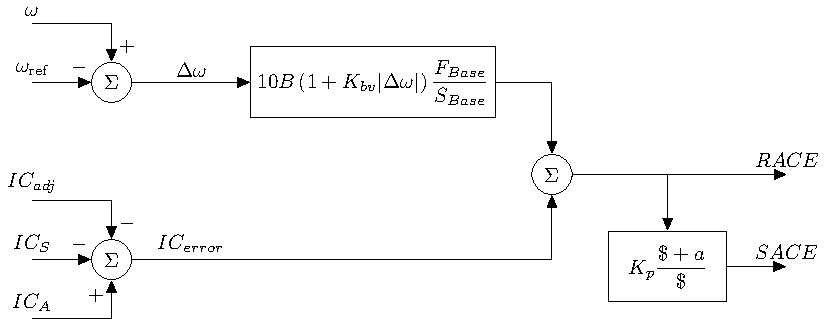
\includegraphics[width=\linewidth]{sections/agc/200722-AGCblockdiagram-p1}
	\caption{AGC calculation of $RACE$ and $SACE$.}
	\label{fig: agc block diagram 1}
\end{figure}%\vspace{-1 em}

\pagebreak
$RACE$ and $SACE$ are calculated every simulation time step, however
distribution of $SACE$ is determined by the user defined \verb|startTime| and \verb|actionTime| variables.
Assuming action, the conditional $\Delta\omega$ logic is processed before adjusting the \verb|aceSig| value which is then gained to become \verb|ace2dist|.

\begin{figure}[!h]
	\centering
	\footnotesize
	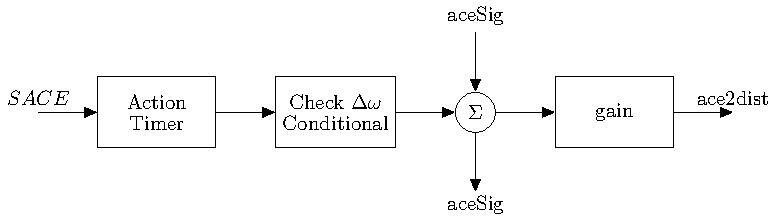
\includegraphics[width=\linewidth]{sections/agc/200722-AGCblockdiagram-p2}
	\caption{AGC calculation of $ace2dist$.}
	\label{fig: agc block diagram 2}
\end{figure}%\vspace{-1 em}

The \verb|ace2dist| value is distributed to all controlled generators associated with the AGC model according to their respective participation factor \verb|pF|.
Each \verb|ctrlGen| has a unique low pass filter to allow for different `ramping' of signals to individual machines.
The output of the low pass filter is gained by -1 and added to the existing associated governor \verb|tg_sig| value to drive ACE to zero.

\begin{figure}[!h]
	\centering
	\footnotesize
	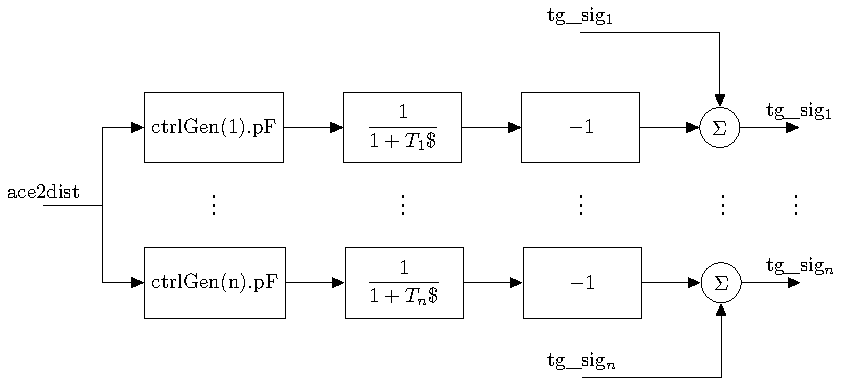
\includegraphics[width=\linewidth]{sections/agc/200722-AGCblockdiagram-p3}
	\caption{AGC handling of $ace2dist$ to individual governor signals.}
	\label{fig: agc block diagram 3}
\end{figure}%\vspace{-1 em}
